\documentclass[conference]{IEEEtran}
\usepackage{filecontents,lipsum}
\usepackage[noadjust]{cite}
\usepackage{graphicx}
\usepackage{mathtools}
\usepackage{subfig}
\usepackage{dcolumn}
\usepackage{booktabs}
\usepackage[table]{xcolor}
\usepackage{ragged2e}
\graphicspath{ {images/}}


\begin{filecontents*}{references.bib}
@INPROCEEDINGS{1199054,
author={S. G. Wysoski and M. V. Lamar and S. Kuroyanagi and A. Iwata},
booktitle={Neural Information Processing, 2002. ICONIP '02. Proceedings of the 9th International Conference on},
title={A rotation invariant approach on static-gesture recognition using boundary histograms and neural networks},
year={2002},
volume={4},
pages={2137-2141 vol.4},
keywords={feature extraction;gesture recognition;neural nets;American Sign Language;complexity;fast search start point algorithm;feature extraction;gesture postures;gesture recognition;pattern recognition;rotation invariance property;rotation invariant;Data mining;Eyes;Fingers;Histograms;Humans;Neural networks;Pattern recognition;Principal component analysis;Robustness;Shape},
doi={10.1109/ICONIP.2002.1199054},
month={Nov},}

@inproceedings{Murakami:1991:GRU:108844.108900,
author = {Murakami, Kouichi and Taguchi, Hitomi},
title = {Gesture Recognition Using Recurrent Neural Networks},
booktitle = {Proceedings of the SIGCHI Conference on Human Factors in Computing Systems},
series = {CHI '91},
year = {1991},
isbn = {0-89791-383-3},
location = {New Orleans, Louisiana, USA},
pages = {237--242},
numpages = {6},
url = {http://doi.acm.org/10.1145/108844.108900},
doi = {10.1145/108844.108900},
acmid = {108900},
publisher = {ACM},
address = {New York, NY, USA},
}

@inproceedings{freeman1995orientation,
title={Orientation histograms for hand gesture recognition},
author={Freeman, William T and Roth, Michal},
booktitle={International workshop on automatic face and gesture recognition},
volume={12},
pages={296--301},
year={1995}
}

@article{vishwakarma2015efficient,
  title={An efficient interpretation of hand gestures to control smart interactive television},
  author={Vishwakarma, DK and Kapoor, R},
  journal={Int. J. Comput. Vis. Robot},
  pages={1--18},
  year={2015}
}

@INPROCEEDINGS{7279962,
author={D. K. Vishwakarma and R. Maheshwari and R. Kapoor},
booktitle={2015 Fifth International Conference on Communication Systems and Network Technologies},
title={An Efficient Approach for the Recognition of Hand Gestures from Very Low Resolution Images},
year={2015},
pages={467-471},
keywords={gesture recognition;image enhancement;image reconstruction;image resolution;digital images;gesture recognition;hand gestures;image enhancement;image recognition;image reconstruction;image resolution;Accuracy;Gesture recognition;Gray-scale;Image recognition;Image resolution;Thumb;geomectry;hand gesture;low resolution;mask generation;recognition},
doi={10.1109/CSNT.2015.84},
month={April},}

@INPROCEEDINGS{6481804,
author={D. K. Vishwakarma and R. Kapoor},
booktitle={2012 4th International Conference on Intelligent Human Computer Interaction (IHCI)},
title={Simple and intelligent system to recognize the expression of speech-disabled person},
year={2012},
pages={1-6},
keywords={binary sequences;computer vision;emotion recognition;feature extraction;handicapped aids;image classification;palmprint recognition;video cameras;Otsu method;binary image;binary sequence;camera;computer vision;disk storage;hand gesture recognition;image conversion;intelligent system;rule based classification approach;shape based feature extraction;speech disabled person expression recognition;thumb;Computers;Feature extraction;Gesture recognition;Image color analysis;Image segmentation;Thumb;Hand gesture recognition;feature extraction;shape based features},
doi={10.1109/IHCI.2012.6481804},
month={Dec},}


@article{barczak2011new,
  title={A new 2D static hand gesture colour image dataset for asl gestures},
  author={Barczak, ALC and Reyes, NH and Abastillas, M and Piccio, A and Susnjak, T},
  year={2011},
  publisher={Massey University}
}

@inproceedings{Avraam2014StaticGR,
  title={Static Gesture Recognition Combining Graph and Appearance Features},
  author={Marimpis Avraam},
  year={2014}
}

@inproceedings{kumar2014static,
  title={Static hand gesture recognition using stacked denoising sparse autoencoders},
  author={Kumar, Varun and Nandi, Gora Chand and Kala, Rahul},
  booktitle={Contemporary Computing (IC3), 2014 Seventh International Conference on},
  pages={99--104},
  year={2014},
  organization={IEEE}
}


@article{khan2012hand,
  title={Hand gesture recognition: a literature review},
  author={Khan, Rafiqul Zaman and Ibraheem, Noor Adnan},
  journal={International journal of artificial Intelligence \& Applications},
  volume={3},
  number={4},
  pages={161},
  year={2012},
  publisher={Academy \& Industry Research Collaboration Center (AIRCC)}
}


@INPROCEEDINGS{7813732,
author={D. K. Vishwakarma and Priyadarshani and K. Singh},
booktitle={2016 International Conference on Computing, Communication and Automation (ICCCA)},
title={A framework for recognition of hand gesture in static postures},
year={2016},
pages={294-298},
keywords={Gabor filters;feature extraction;gesture recognition;gradient methods;image colour analysis;image segmentation;pose estimation;support vector machines;Gabor filter;PHOG;SVM;YCbCr color model;hand gesture recognition framework;hand image region segmentation;pyramid histogram of oriented gradients;saliency image formation;saliency map;skin region detection;skin saliency image spatial distribution;static hand posture images;support vector machine;texture feature extraction;Feature extraction;Gabor filters;Histograms;Image color analysis;Image segmentation;Shape;Skin;Gabor filter;Pyramid histogram of oriented gradients;Static hand gesture;saliency map},
doi={10.1109/CCAA.2016.7813732},
month={April},}

@inproceedings{droeschel2011learning,
  title={Learning to interpret pointing gestures with a time-of-flight camera},
  author={Droeschel, David and St{\"u}ckler, J{\"o}rg and Behnke, Sven},
  booktitle={Proceedings of the 6th international conference on Human-robot interaction},
  pages={481--488},
  year={2011},
  organization={ACM}
}

@article{shotton2013real,
  title={Real-time human pose recognition in parts from single depth images},
  author={Shotton, Jamie and Sharp, Toby and Kipman, Alex and Fitzgibbon, Andrew and Finocchio, Mark and Blake, Andrew and Cook, Mat and Moore, Richard},
  journal={Communications of the ACM},
  volume={56},
  number={1},
  pages={116--124},
  year={2013},
  publisher={ACM}
}

@inproceedings{regenbrecht2013leap,
  title={A leap-supported, hybrid AR interface approach},
  author={Regenbrecht, Holger and Collins, Jonny and Hoermann, Simon},
  booktitle={Proceedings of the 25th Australian Computer-Human Interaction Conference: Augmentation, Application, Innovation, Collaboration},
  pages={281--284},
  year={2013},
  organization={ACM}
}

@article{cheng2016survey,
  title={Survey on 3D Hand Gesture Recognition},
  author={Cheng, Hong and Yang, Lu and Liu, Zicheng},
  journal={IEEE Transactions on Circuits and Systems for Video Technology},
  volume={26},
  number={9},
  pages={1659--1673},
  year={2016},
  publisher={IEEE}
}


\end{filecontents*}

%\bibliographystyle{plain}
% Some Computer Society conferences also require the compsoc mode option,
% but others use the standard conference format.
%
% If IEEEtran.cls has not been installed into the LaTeX system files,
% manually specify the path to it like:
% \documentclass[conference]{../sty/IEEEtran}





% Some very useful LaTeX packages include:
% (uncomment the ones you want to load)


% *** MISC UTILITY PACKAGES ***
%
%\usepackage{ifpdf}
% Heiko Oberdiek's ifpdf.sty is very useful if you need conditional
% compilation based on whether the output is pdf or dvi.
% usage:
% \ifpdf
%   % pdf code
% \else
%   % dvi code
% \fi
% The latest version of ifpdf.sty can be obtained from:
% http://www.ctan.org/pkg/ifpdf
% Also, note that IEEEtran.cls V1.7 and later provides a builtin
% \ifCLASSINFOpdf conditional that works the same way.
% When switching from latex to pdflatex and vice-versa, the compiler may
% have to be run twice to clear warning/error messages.









% *** GRAPHICS RELATED PACKAGES ***
%
\ifCLASSINFOpdf
  % \usepackage[pdftex]{graphicx}
  % declare the path(s) where your graphic files are
  % \graphicspath{{../pdf/}{../jpeg/}}
  % and their extensions so you won't have to specify these with
  % every instance of \includegraphics
  % \DeclareGraphicsExtensions{.pdf,.jpeg,.png}
\else
  % or other class option (dvipsone, dvipdf, if not using dvips). graphicx
  % will default to the driver specified in the system graphics.cfg if no
  % driver is specified.
  % \usepackage[dvips]{graphicx}
  % declare the path(s) where your graphic files are
  % \graphicspath{{../eps/}}
  % and their extensions so you won't have to specify these with
  % every instance of \includegraphics
  % \DeclareGraphicsExtensions{.eps}
\fi
% graphicx was written by David Carlisle and Sebastian Rahtz. It is
% required if you want graphics, photos, etc. graphicx.sty is already
% installed on most LaTeX systems. The latest version and documentation
% can be obtained at: 
% http://www.ctan.org/pkg/graphicx
% Another good source of documentation is "Using Imported Graphics in
% LaTeX2e" by Keith Reckdahl which can be found at:
% http://www.ctan.org/pkg/epslatex
%
% latex, and pdflatex in dvi mode, support graphics in encapsulated
% postscript (.eps) format. pdflatex in pdf mode supports graphics
% in .pdf, .jpeg, .png and .mps (metapost) formats. Users should ensure
% that all non-photo figures use a vector format (.eps, .pdf, .mps) and
% not a bitmapped formats (.jpeg, .png). The IEEE frowns on bitmapped formats
% which can result in "jaggedy"/blurry rendering of lines and letters as
% well as large increases in file sizes.
%
% You can find documentation about the pdfTeX application at:
% http://www.tug.org/applications/pdftex





% *** MATH PACKAGES ***
%
%\usepackage{amsmath}
% A popular package from the American Mathematical Society that provides
% many useful and powerful commands for dealing with mathematics.
%
% Note that the amsmath package sets \interdisplaylinepenalty to 10000
% thus preventing page breaks from occurring within multiline equations. Use:
%\interdisplaylinepenalty=2500
% after loading amsmath to restore such page breaks as IEEEtran.cls normally
% does. amsmath.sty is already installed on most LaTeX systems. The latest
% version and documentation can be obtained at:
% http://www.ctan.org/pkg/amsmath





% *** SPECIALIZED LIST PACKAGES ***
%
%\usepackage{algorithmic}
% algorithmic.sty was written by Peter Williams and Rogerio Brito.
% This package provides an algorithmic environment fo describing algorithms.
% You can use the algorithmic environment in-text or within a figure
% environment to provide for a floating algorithm. Do NOT use the algorithm
% floating environment provided by algorithm.sty (by the same authors) or
% algorithm2e.sty (by Christophe Fiorio) as the IEEE does not use dedicated
% algorithm float types and packages that provide these will not provide
% correct IEEE style captions. The latest version and documentation of
% algorithmic.sty can be obtained at:
% http://www.ctan.org/pkg/algorithms
% Also of interest may be the (relatively newer and more customizable)
% algorithmicx.sty package by Szasz Janos:
% http://www.ctan.org/pkg/algorithmicx




% *** ALIGNMENT PACKAGES ***
%
%\usepackage{array}
% Frank Mittelbach's and David Carlisle's array.sty patches and improves
% the standard LaTeX2e array and tabular environments to provide better
% appearance and additional user controls. As the default LaTeX2e table
% generation code is lacking to the point of almost being broken with
% respect to the quality of the end results, all users are strongly
% advised to use an enhanced (at the very least that provided by array.sty)
% set of table tools. array.sty is already installed on most systems. The
% latest version and documentation can be obtained at:
% http://www.ctan.org/pkg/array


% IEEEtran contains the IEEEeqnarray family of commands that can be used to
% generate multiline equations as well as matrices, tables, etc., of high
% quality.




% *** SUBFIGURE PACKAGES ***
%\ifCLASSOPTIONcompsoc
%  \usepackage[caption=false,font=normalsize,labelfont=sf,textfont=sf]{subfig}
%\else
%  \usepackage[caption=false,font=footnotesize]{subfig}
%\fi
% subfig.sty, written by Steven Douglas Cochran, is the modern replacement
% for subfigure.sty, the latter of which is no longer maintained and is
% incompatible with some LaTeX packages including fixltx2e. However,
% subfig.sty requires and automatically loads Axel Sommerfeldt's caption.sty
% which will override IEEEtran.cls' handling of captions and this will result
% in non-IEEE style figure/table captions. To prevent this problem, be sure
% and invoke subfig.sty's "caption=false" package option (available since
% subfig.sty version 1.3, 2005/06/28) as this is will preserve IEEEtran.cls
% handling of captions.
% Note that the Computer Society format requires a larger sans serif font
% than the serif footnote size font used in traditional IEEE formatting
% and thus the need to invoke different subfig.sty package options depending
% on whether compsoc mode has been enabled.
%
% The latest version and documentation of subfig.sty can be obtained at:
% http://www.ctan.org/pkg/subfig




% *** FLOAT PACKAGES ***
%
%\usepackage{fixltx2e}
% fixltx2e, the successor to the earlier fix2col.sty, was written by
% Frank Mittelbach and David Carlisle. This package corrects a few problems
% in the LaTeX2e kernel, the most notable of which is that in current
% LaTeX2e releases, the ordering of single and double column floats is not
% guaranteed to be preserved. Thus, an unpatched LaTeX2e can allow a
% single column figure to be placed prior to an earlier double column
% figure.
% Be aware that LaTeX2e kernels dated 2015 and later have fixltx2e.sty's
% corrections already built into the system in which case a warning will
% be issued if an attempt is made to load fixltx2e.sty as it is no longer
% needed.
% The latest version and documentation can be found at:
% http://www.ctan.org/pkg/fixltx2e


%\usepackage{stfloats}
% stfloats.sty was written by Sigitas Tolusis. This package gives LaTeX2e
% the ability to do double column floats at the bottom of the page as well
% as the top. (e.g., "\begin{figure*}[!b]" is not normally possible in
% LaTeX2e). It also provides a command:
%\fnbelowfloat
% to enable the placement of footnotes below bottom floats (the standard
% LaTeX2e kernel puts them above bottom floats). This is an invasive package
% which rewrites many portions of the LaTeX2e float routines. It may not work
% with other packages that modify the LaTeX2e float routines. The latest
% version and documentation can be obtained at:
% http://www.ctan.org/pkg/stfloats
% Do not use the stfloats baselinefloat ability as the IEEE does not allow
% \baselineskip to stretch. Authors submitting work to the IEEE should note
% that the IEEE rarely uses double column equations and that authors should try
% to avoid such use. Do not be tempted to use the cuted.sty or midfloat.sty
% packages (also by Sigitas Tolusis) as the IEEE does not format its papers in
% such ways.
% Do not attempt to use stfloats with fixltx2e as they are incompatible.
% Instead, use Morten Hogholm'a dblfloatfix which combines the features
% of both fixltx2e and stfloats:
%
% \usepackage{dblfloatfix}
% The latest version can be found at:
% http://www.ctan.org/pkg/dblfloatfix




% *** PDF, URL AND HYPERLINK PACKAGES ***
%
%\usepackage{url}
% url.sty was written by Donald Arseneau. It provides better support for
% handling and breaking URLs. url.sty is already installed on most LaTeX
% systems. The latest version and documentation can be obtained at:
% http://www.ctan.org/pkg/url
% Basically, \url{my_url_here}.




% *** Do not adjust lengths that control margins, column widths, etc. ***
% *** Do not use packages that alter fonts (such as pslatex).         ***
% There should be no need to do such things with IEEEtran.cls V1.6 and later.
% (Unless specifically asked to do so by the journal or conference you plan
% to submit to, of course. )


% correct bad hyphenation here
\hyphenation{op-tical net-works semi-conduc-tor}


\begin{document}
%
% paper title
% Titles are generally capitalized except for words such as a, an, and, as,
% at, but, by, for, in, nor, of, on, or, the, to and up, which are usually
% not capitalized unless they are the first or last word of the title.
% Linebreaks \\ can be used within to get better formatting as desired.
% Do not put math or special symbols in the title.
\title{A Static Hand Gesture Recognition System to Recognize the Total number of Fingers}


% author names and affiliations
% use a multiple column layout for up to three different
% affiliations


\author{\IEEEauthorblockN{D.K. Vishwakarma\IEEEauthorrefmark{1}  Sahib Majithia\IEEEauthorrefmark{2} Nikhil Kumar Mishra\IEEEauthorrefmark{3}}
\IEEEauthorblockA{Department of Electronics and Communication Engineering,
\\Delhi Technological University\\
New Delhi, India\\
Email: \IEEEauthorrefmark{1}dvishwakarma@gmail.com ,\IEEEauthorrefmark{2}sahibmajithia@gmail.com,
\IEEEauthorrefmark{3}nkmishra1997@gmail.com}}

% conference papers do not typically use \thanks and this command
% is locked out in conference mode. If really needed, such as for
% the acknowledgment of grants, issue a \IEEEoverridecommandlockouts
% after \documentclass

% for over three affiliations, or if they all won't fit within the width
% of the page, use this alternative format:
% 
%\author{\IEEEauthorblockN{Michael Shell\IEEEauthorrefmark{1},
%Homer Simpson\IEEEauthorrefmark{2},
%James Kirk\IEEEauthorrefmark{3}, 
%Montgomery Scott\IEEEauthorrefmark{3} and
%Eldon Tyrell\IEEEauthorrefmark{4}}
%\IEEEauthorblockA{\IEEEauthorrefmark{1}School of Electrical and Computer Engineering\\
%Georgia Institute of Technology,
%Atlanta, Georgia 30332--0250\\ Email: see http://www.michaelshell.org/contact.html}
%\IEEEauthorblockA{\IEEEauthorrefmark{2}Twentieth Century Fox, Springfield, USA\\
%Email: homer@thesimpsons.com}
%\IEEEauthorblockA{\IEEEauthorrefmark{3}Starfleet Academy, San Francisco, California 96678-2391\\
%Telephone: (800) 555--1212, Fax: (888) 555--1212}
%\IEEEauthorblockA{\IEEEauthorrefmark{4}Tyrell Inc., 123 Replicant Street, Los Angeles, California 90210--4321}}




% use for special paper notices
%\IEEEspecialpapernotice{(Invited Paper)}




% make the title area
\maketitle

% As a general rule, do not put math, special symbols or citations
% in the abstract
\begin{abstract}
The main purpose of gesture recognition systems is to understand important expressions of motion by humans which involve hands, head, face, arms, or body.It is of major importance in designing an expert interface between humans and computers.We take into account the two possible fixed geometries to work on. The proposed methods follow the procedure of Preprocessing: which helps with noise removal and image enhancement; Segmentation of hand region: uses skin likelihood method to extract skin color; Feature extraction: Morphological and geometry based functions are used to extract the fingers; and active fingers are counted by method of Rule based Classification. In order to test performance, an experiment is conducted using standard and a self-generated dataset of images. The accuracy achieved on these dataset is greater than on similar state of arts. \\ \\

\begin{IEEEkeywords}
\textit{Hand Gestures, Skin Segmentation, Active Fingers, Finger Count, Mask Generation, Recognition, Low Resolution}

\end{IEEEkeywords}
 
\end{abstract}

% no keywords




% For peer review papers, you can put extra information on the cover
% page as needed:
% \ifCLASSOPTIONpeerreview
% \begin{center} \bfseries EDICS Category: 3-BBND \end{center}
% \fi
%
% For peerreview papers, this IEEEtran command inserts a page break and
% creates the second title. It will be ignored for other modes.
\IEEEpeerreviewmaketitle



\section{Introduction}
An efficient human computer interplay is prominent in the present day framework of interactive and smart computing. Gesture recognition is the leading progress in this direction.
Gesture recognition is the substantiated analysis of a human movement by a computing device

 There are methods which used extra hardware accessories such as color markers and data glove devices to easily extract a complete classification of gesture traits for identification \cite{1199054} . Neural Network classifiers have been implemented for gestures classification \cite{Murakami:1991:GRU:108844.108900} but it is long-drawn out and as the amount of training data grows, the time necessitated for classification is extended too.Orientation histogram method \cite{freeman1995orientation} has some inherent difficulties which are; different gestures could have related orientation histograms, and related gestures might have distinctive orientation histograms. Other methods based on the appearance of the hand use the color of our skin to section the hand and obtain necessary features, these methods are considered natural, simple and less computationally costly compared with methods mentioned before \cite{1199054} .

Three dimensional hand model based approaches \cite{cheng2016survey} are earning interest in the domain of Gesture Recognition.		Three dimensional hand model based approaches \cite{cheng2016survey} are gaining interest in the field of Gesture Recognition.
The popular gesture sensors used presently are:

A. Time-of-Flight Sensors:
ToF-based 3D hand gesture recognition system uses point gestures to control a robot \cite{droeschel2011learning}.

B. Kinect

 1) skeletonbased recognition \cite{shotton2013real} and 
 
 2) depth-based recognition.

C. Leap Motion: Leap Motion is a newly released sensor that focuses on the accurate 3D hand positioning. It concentrates on a specific region and has gained prevalence over Kinect sensor concerning better accuracy \cite{regenbrecht2013leap}.

This paper proposes two methods for counting the number of active fingers. These are proposed based on the geometric facts of the hand region. 

Since the proposed method works on geometric properties and does not require any extracted features; it works well on low-resolution images which is a great advantage for developers regarding data storage.

The algorithm first helps with skin segmentation from the region of interest. Further, the number of active fingers are counted after operating them with a range of morphological operations.
In this paper section 2 and 3 describe the algorithms proposed. Further sections discuss the Results (4), Conclusions (5) and Future scope (6) of our work.


%This paper is composed into following following sections blah!

%sectoin{Theory}

\section{Hand Segmentation}

Skin segmentation obtains the hand region. The skin segmentation has been applied correctly to Region of Interest of hand region. This does not cause susceptibility as the Region of Interest can be easily extracted by different depth estimation strategies, which include:

Active methods:
Light-based depth estimation/Pattern projection/Ultrasounds based methods

Passive methods:
Monocular depth estimation/Image structure/Points tracking or Optical flow/ Multiview solutions for the depth estimation

The Region of interest can also be extracted by using instruments like Kinect which uses an RGB camera with a depth sensor.

We have used gestures G1, G2, G3, G4 and G5.
\begin{figure}[!h]
\begin{tabular}{ccccc}
\subfloat[G1]{
\includegraphics[width = 0.55in]{ges1}} &
\subfloat[G2]{
\includegraphics[width = 0.55in]{ges2}} &
\subfloat[G3]{
\includegraphics[width = 0.55in]{ges3}} &
\subfloat[G4]{
\includegraphics[width = 0.55in]{ges4}} &
\subfloat[G5]{
\includegraphics[width = 0.55in]{ges5}}
\end{tabular}
\caption{Gestures used with extracted ROI}
\end{figure}

\subsection{SKIN SEGMENTATION}

The most important part of hand gesture recognition is the skin segmentation. Segmentation accuracy determines the eventual success or failure of an automated analysis procedure.For segmentation, we first convert the RGB colored image into the YCbCr color model.

The transformation of the original RGB colour image is done using
the following equations:

\begin{equation}
 Y = 0.2990R + 0.5870G + 0.1140B
\end{equation}
\begin{equation}
 Cb = -0.1687R - 0.3313G + 0.5000B
\end{equation}
\begin{equation}
 Cr = 0.5000R - 0.4187G - 0.0813B
\end{equation}


The mean values of chrominance components are used to extract the skin color of the hand by dropping the luminance component because the variation in skin color is more in intensity than in chrominance. In YCbCr color space, the components Cb and Cr represent the chrominance and component Y accounts for the luminance.

In the earlier works, the YCbCr color model has been used by a basic mathematic operation of thresholding on chromaticity and luminance values. No method has yet been settled which determines the thresholding accurately.So, alternatively, we use a modified approach called a skin likelihood model for skin segmentation.

This model is devised from the maximum likelihood paradigm, which has two parameters: covariance matrix and mean vector that maximizes the likelihood function. The Gaussian likelihood function \cite{vishwakarma2015efficient} has unique maxima, and the parameters  covariance matrix ($\Upsilon$) and mean vector($\xi$) is calculated as:

\begin{equation}
\begin{aligned}
\Upsilon_i = \frac{1}{n} & \sum_{k=1}^\infty y_k
\end{aligned}
\end{equation}
Where i $\in$ \{Cb,Cr\}  Cb and Cr are the values of chrominance in YCbCr color space.
\begin{equation}
\begin{aligned}
\xi = \frac{1}{n} & \sum_{k=1}^\infty \left(y_k - \Upsilon \right)\left(y_k - \Upsilon \right)^T
\end{aligned}
\end{equation}
The probability distribution of skin class can be written as:
\begin{equation}
\begin{aligned}
p(\frac{y}{skin}) =  g(y,\Upsilon,\xi)
\end{aligned}
\end{equation}

\begin{equation}
\begin{aligned}
g(y,\Upsilon,\xi) =  \frac{1}{(2\pi)^{\frac{d}{2}}\left(det\left(\xi \right)\right)^\frac{1}{2}} \times exp(-\frac{1}{2}\delta^2)
\end{aligned}
\end{equation}

Where d is the dimension of the feature vector, and \linebreak
$\delta^2 =(y - \Upsilon_i)\xi^{-1}(y - \Upsilon_i)^T $ .From equation 4, the pixels can be classified as skin and non-skin color pixels by using the decision boundary. The probability density distribution of the formed Gaussian model is represented in figure:
\begin{figure}[h!]
	\centering
	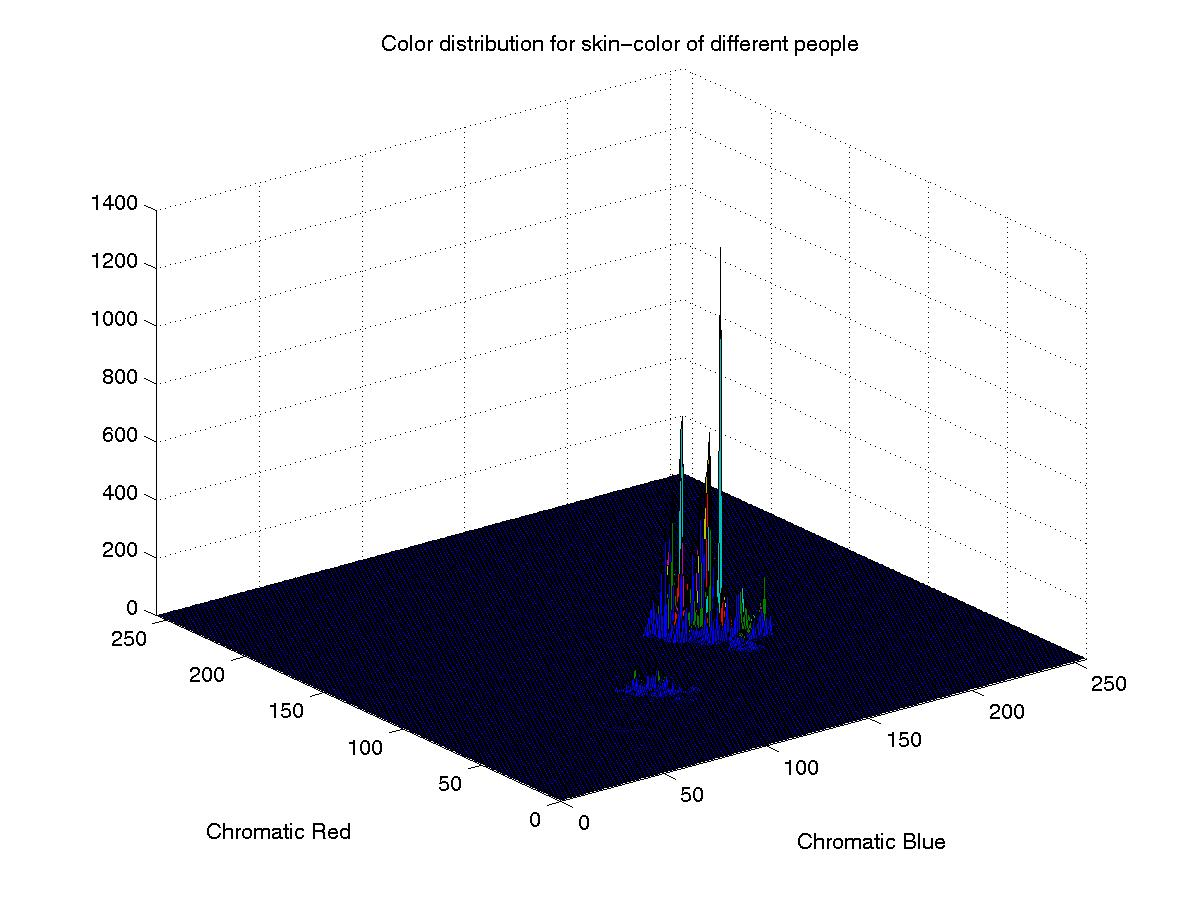
\includegraphics[width = 6.5cm, height = 5cm]{skincolor}
	\caption{ Graph describing variation of skin tones of human race in Chromatic colour model}
\end{figure}
Plotting a Gaussian Curve for this variation yields the Graph in figure 3.
\begin{figure}[h!]
	\centering
	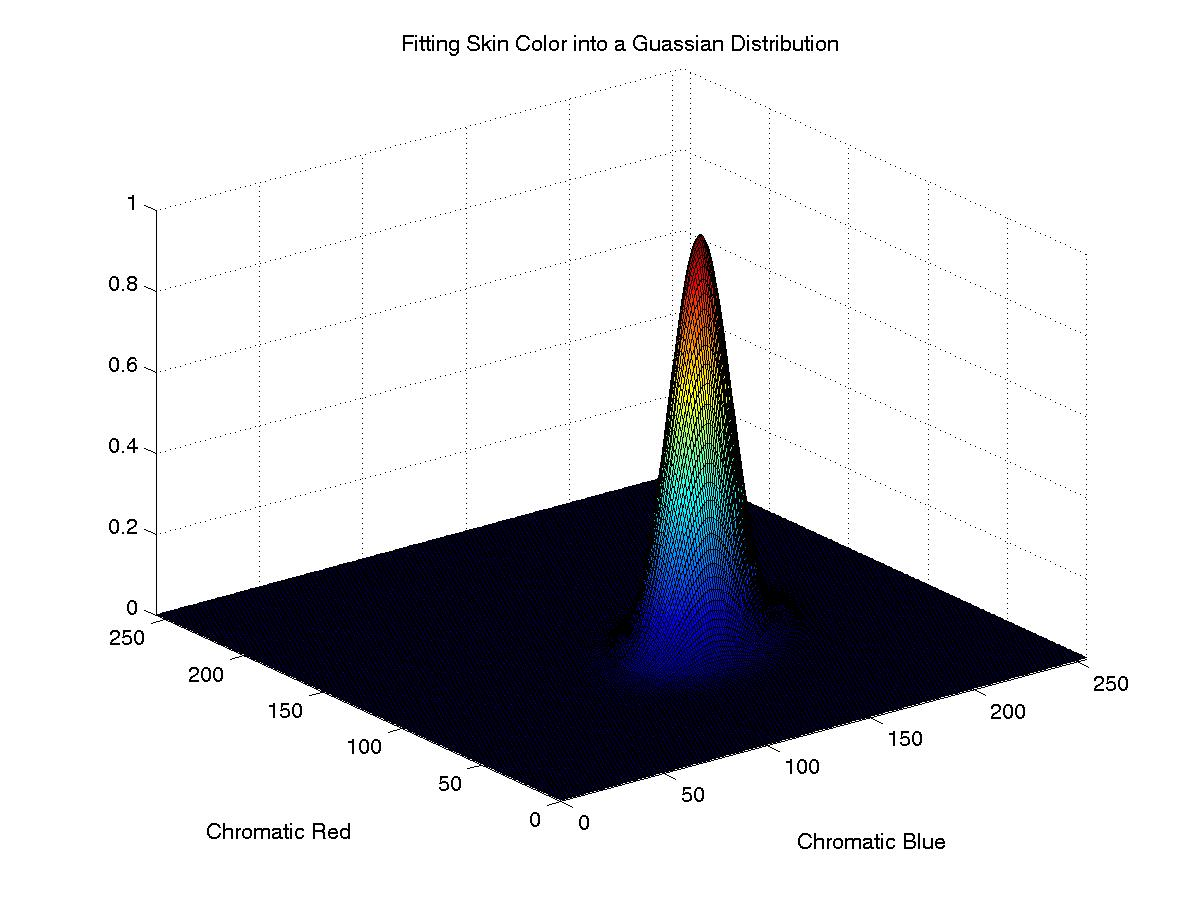
\includegraphics[width = 6.5cm, height = 5cm]{gaussian}
	\caption{Gaussian curve of variations in Fig.1}
\end{figure}

This Method has a great accuracy and calibration advantage over the YCbCr model and is thus more user-friendly. It can be calibrated for all fairer to darker skins with just a change in input skin section (which was trained for the Gaussian ); in contrast to change in Cb and Cr values which demand a technical blueprint.

\subsection{PSEUDO CODE:}
\begin{flushleft}
$imresize([200 200])$ 

SKIN SEGMENTATION:

$train skin model : $

$function\_outputs[ mean(cr) ,mean(cb), cov(cr,cb)]$

$x = [(cr-r_{mean});(cb-b_{mean})];$

$likely\_skin(i,j) = [power(2*pi*power(det(rbcov),0.5),-1)]*exp(-0.5* y'*inv(rbcov)* y);$

For every pixel we calculate :

$likely\_skin(i,j) = [power(2*pi*power(det(rbcov),0.5),-1)]*exp(-0.5*y'*inv(rbcov)*y);$ \% gives the Gaussian of the image. 

$BW = im2bw(likely_skin,thresh); $ \% Morphological operations for segmenting the hand shape accurately

$imclose;imdilate;imfill('holes');$

Find the hand(palm width) 
\end{flushleft}
\begin{figure}[h!]
	\centering
	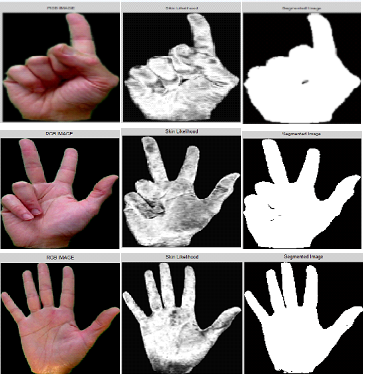
\includegraphics[width = 5.5cm, height = 5.5cm]{grid1}
	%\caption{Gaussian curve of variations in Fig.1}
\end{figure}



\section{PROPOSED METHODS}

\subsection{Method 1: MASKING APPROACH }

After acquiring a binary image of the segmented skin region, we extract the count of active fingers by a distinct system of morphological operations.


\subsubsection{MORPHOLOGY}

Morphology is a comprehensive collection of image processing methods that process images by shapes and contours.

Dilation and Erosion work (at least conceptually) by translating the structuring element to various points in the input image, and examining the projection between the translated kernel coordinates and the input image coordinates.

Mathematically, the main morphological operations we use are denoted as follows:

\paragraph{EROSION}
\begin{equation}
\begin{aligned}
\left(J \ominus K\right) = \left[z|(K)_z\subseteq J \right]\,
\end{aligned}
\end{equation}

%\begin{figure}[h!]
%	\centering
%	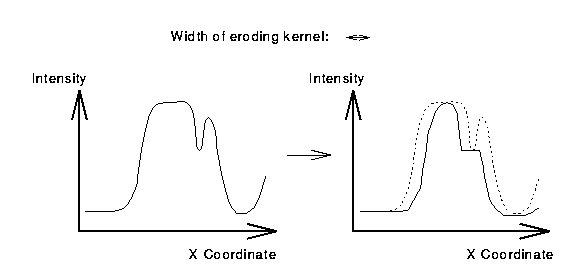
\includegraphics[width = 7cm, height = 4cm]{erosion}
%	%\caption{Gaussian curve of variations in Fig.1}
%\end{figure}

\paragraph{DILATION}
\begin{equation}
\begin{aligned}
\left(J \oplus K\right) =  \left[z|(\widehat{K})_z\cap J \neq \phi \right]\,
\end{aligned}
\end{equation}

imopen:
\begin{equation}
\begin{aligned}
\left(J \hspace{2mm} o\hspace{2mm} K\right) =  \left[\left(J \ominus K \right) \oplus K \right]\,
\end{aligned}
\end{equation}

imclose:
\begin{equation}
\begin{aligned}
\left(J  \cdot  K\right) =  \left[\left(J \oplus K \right) \ominus K \right]\,
\end{aligned}
\end{equation}

%\begin{figure}[h!]
%	\centering
%	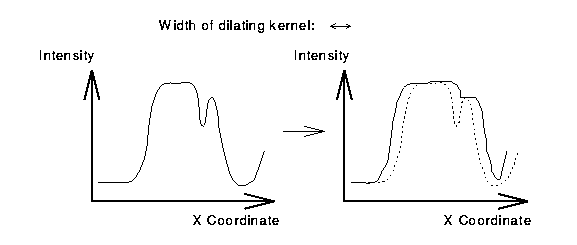
\includegraphics[width = 7cm, height = 4cm]{dilation}
%	%\caption{Gaussian curve of variations in Fig.1}
%\end{figure}

\subsubsection{OPERATIONS}
The palm width calculation is needed for obtaining the finger width.

The finger width lies between 1/3 to 1/4 times the palm width depending on the stretch of fingers.

An erosion filter is then designed which is of the dimension of the finger girth. This filter is employed for erosion on the binary segmented image. Dilation of this image helps obtain the mask (here palm).

Morphological opening, closing, and other fitting operations should be executed to accomplish a noise-free and an explicitly shaped mask.

The subtraction of the mask \cite{7279962} from the binary image provides us the active fingers of the image. Further thresholding for the area of the acquired portions presents us with the precise count of active fingers.


\subsubsection{PSEUDO CODE}

\textbf{Masking Approach}
\begin{flushleft}
3 \textless ratio \textless 4

$erode\_filter=ones(1,floor(width/ratio); $ \% remove small components such as noises and uneroded finger parts
 
$bwareaopen(eroded\_image,40);$ \%dilate to obtain the original palm shape and size. 

$fingers=~palm.*BW$ 

$regionprops \rightarrow$ Area threshholding to count the no. of bounding box to count the number of fingers.

\begin{figure}[h!]
	\centering
	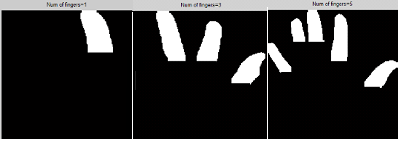
\includegraphics[width = 8cm, height = 3cm]{method1_1}
	%\caption{Gaussian curve of variations in Fig.1}
\end{figure}
\end{flushleft}
\subsection{Method 2: GRADIENT APPROACH}
After acquiring a binary image of the segmented skin region, we extract the count of active fingers by using the information of the change of gradients at the finger-tip region.Once the centroid of the binary image is acquired, we determine the shortest distance to the boundary of the silhoutte from the centroid point. This minimum distance is defined in all directions from the centroid.The area hereafter produced showcases the mask for the binary silhouette.It comprises the palm region of the hand and thus forms the base of the mask  \cite{6481804}.Mask subtraction then gives us the fingertip section in addition to the wrist area.

Gradients are calculated by using filters :

Gx: forward horizontal difference 

Gy: forward vertical difference

\begin{equation}
\begin{aligned}
Gradient = \sqrt{G_x^2 + G_y^2}
\end{aligned}
\end{equation}


We use sobel gradient operator for our method.
\[
  \stackrel{\mbox{$G$x}}{%
    \begin{bmatrix}
    -1 & 0 & +1 \\
    -2 & 0 & +2 \\
    -1 & 0 & +1
    \end{bmatrix}%
  }\ \quad
  \stackrel{\mbox{$G$y}}{%
    \begin{bmatrix}
    -1 & +2 & +1 \\
    0 & 0 & 0 \\
    -1 & -2 & -1
    \end{bmatrix}%
  }
\]


Gradient map of the obtained image is calculated. The geometry of the hand infers that the wrist area has a small change of slope at the boundary region though the change is high for the fingertips.

Thus a suitable threshold is established to segregate the wrist area.

The gradient map is transferred via a low-pass filter to eliminate the noise effects. The low-pass filter also helps identify the false high-gradient-change locations.

The final gradient map is a plot for column locations, and thresholding identifies the count of fingers.

\begin{figure}[!h]
\begin{tabular}{cc}
\subfloat{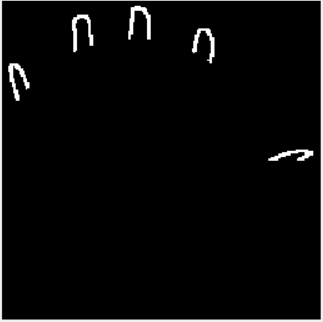
\includegraphics[width = 0.9in]{method2_5}} &
\subfloat{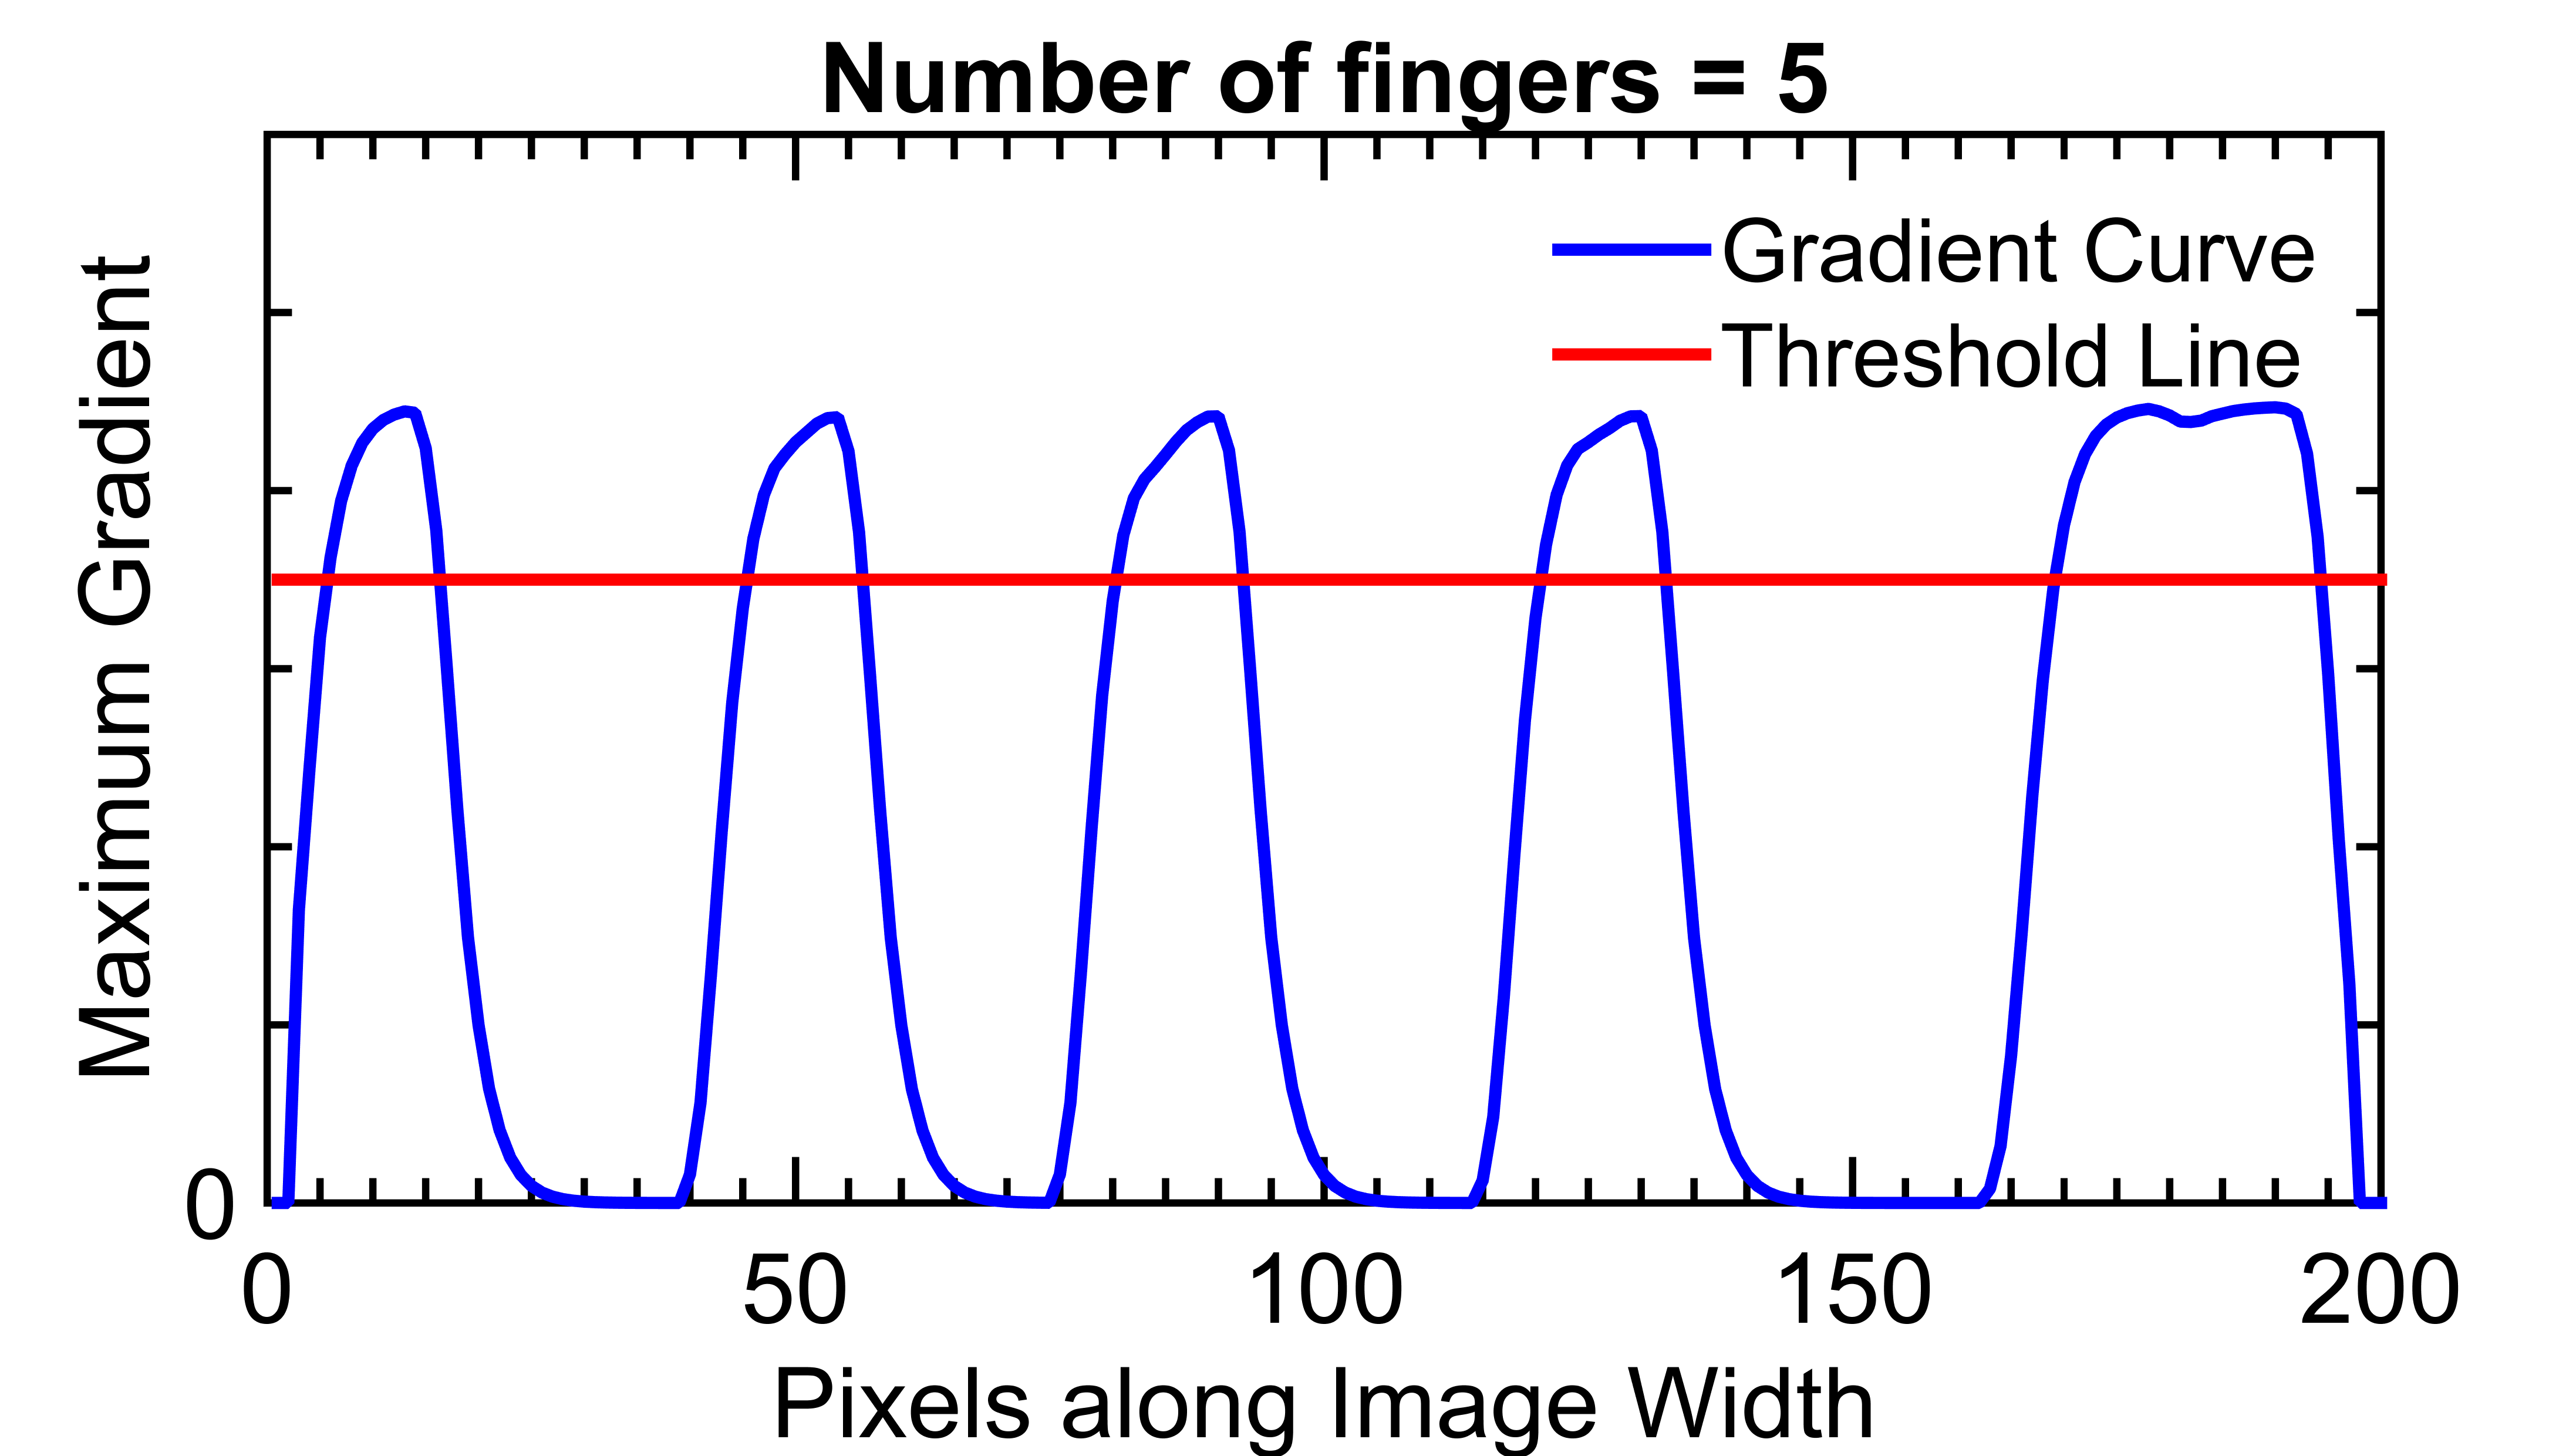
\includegraphics[width = 1.6in]{plot5}}
\end{tabular}
%\caption{Gestures used with extracted ROI}
\end{figure}

\begin{figure}[!h]
\begin{tabular}{cc}
\subfloat{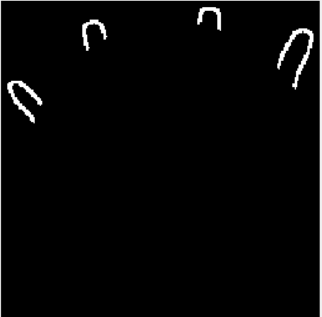
\includegraphics[width = 0.9in]{method2_4}} &
\subfloat{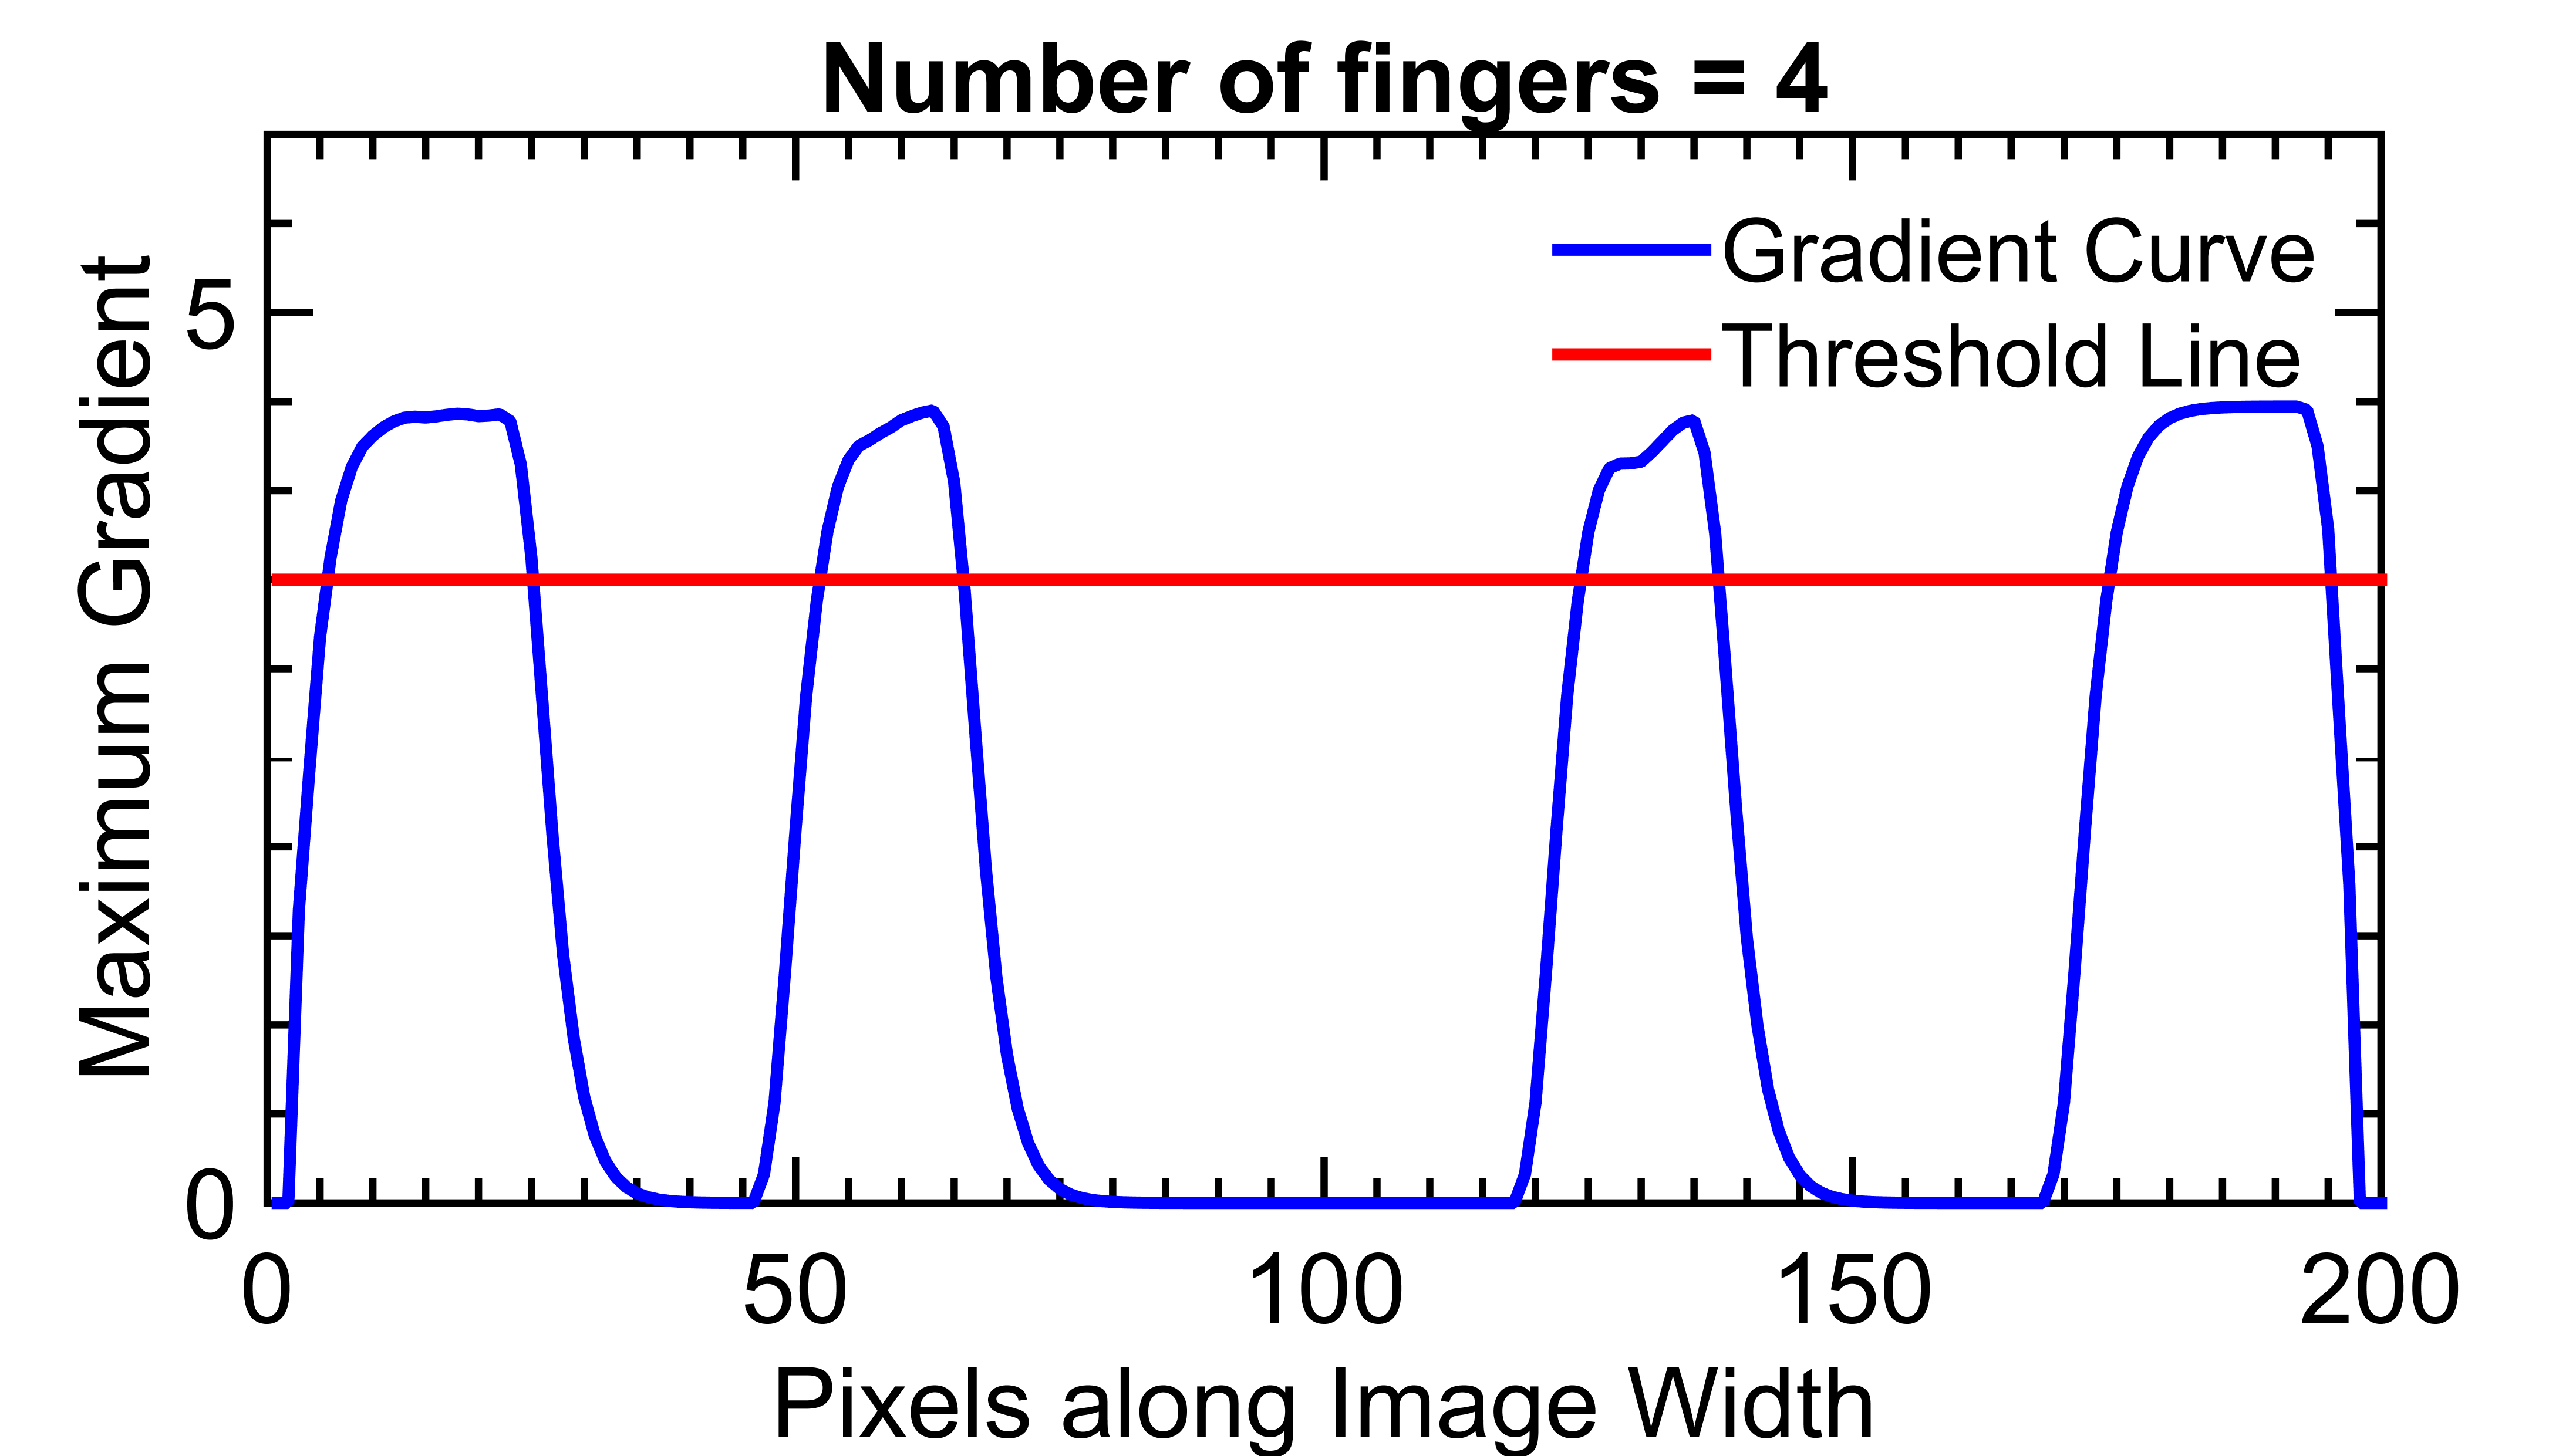
\includegraphics[width = 1.6in]{plot4}}
\end{tabular}
%\caption{Gestures used with extracted ROI}
\end{figure}

\begin{figure}[!h]
\begin{tabular}{cc}
\subfloat{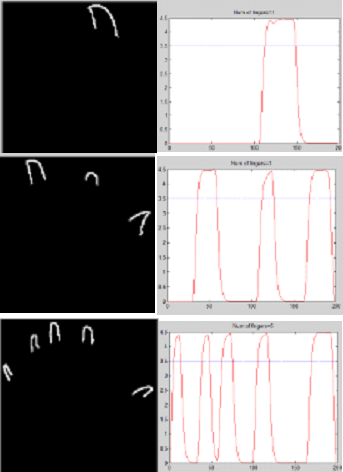
\includegraphics[width = 0.9in]{method2_2}} &
\subfloat{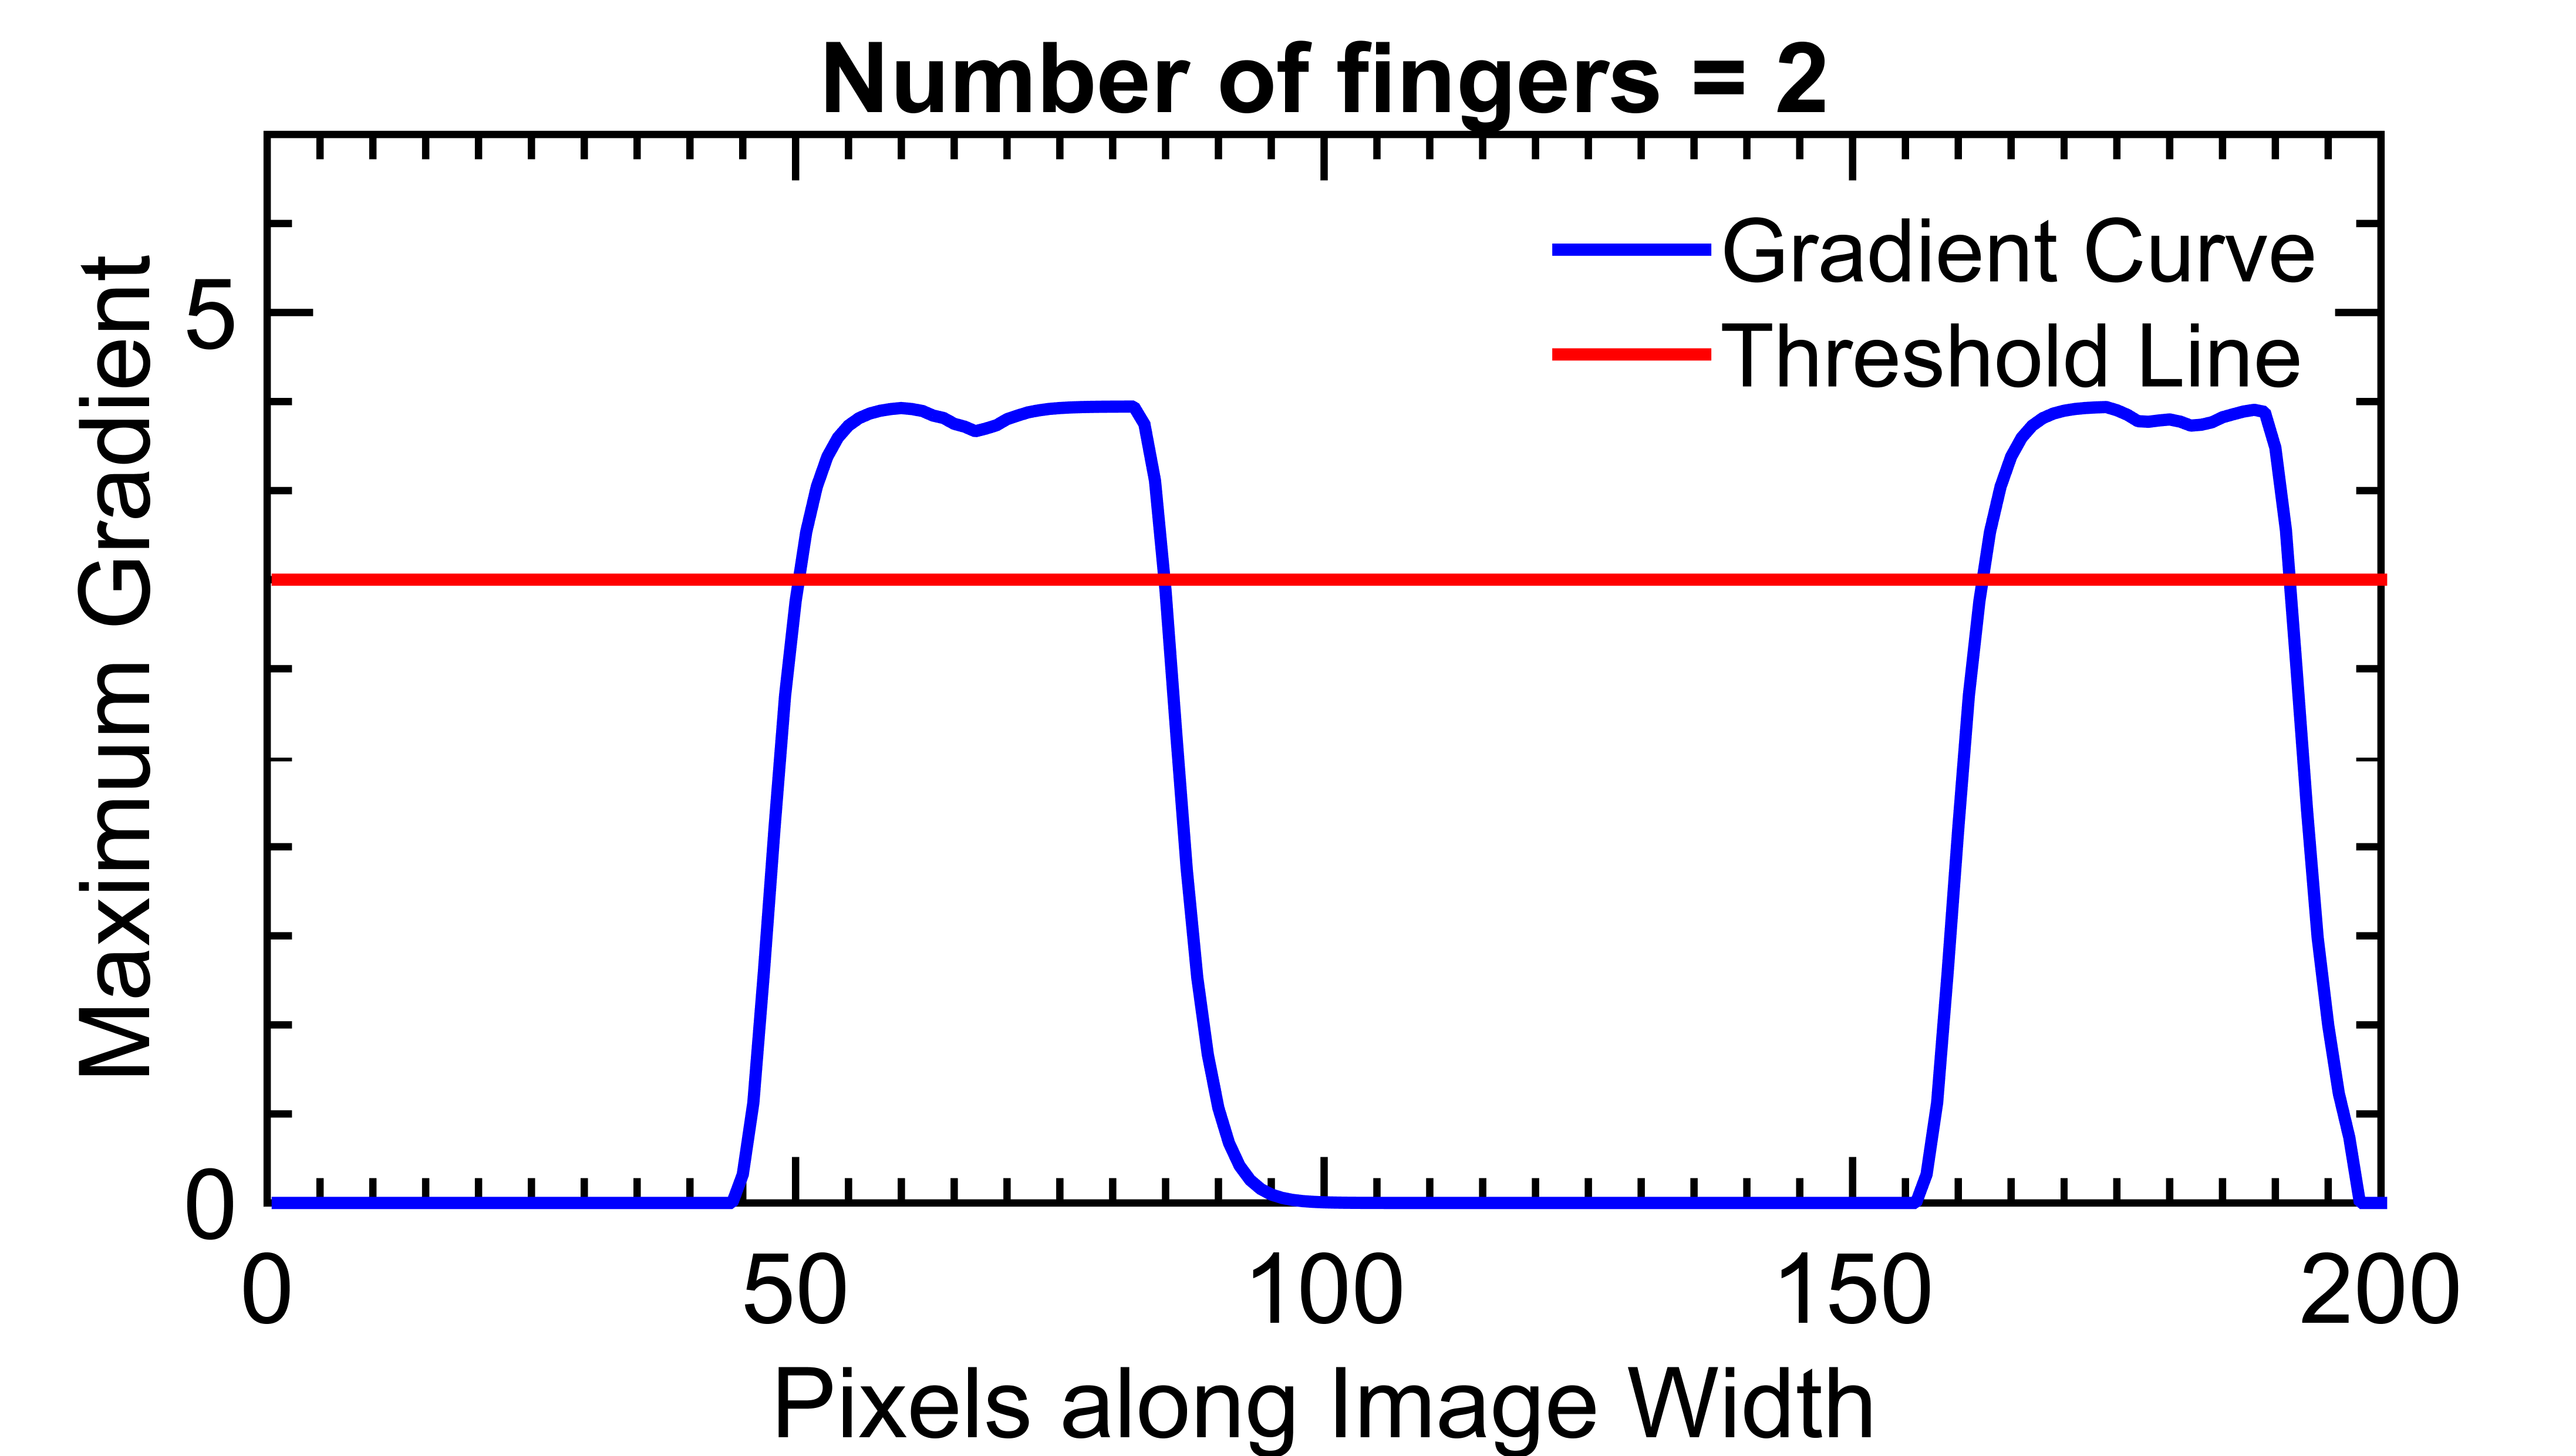
\includegraphics[width = 1.6in]{plot2}}
\end{tabular}
%\caption{Gestures used with extracted ROI}
\end{figure}

\subsubsection{PSEUDO CODE}
\textbf{Gradient Approach}
\begin{flushleft}


$erode\_filter= strel('disk',5);$ \% remove small components such as noises and uneroded finger parts
 
$[Gmag, Gdir] = imgradient(eroded \_ image); $ \% find the change and direction of gradient at the boundary of the entire hand region. 

for $i=1:width$\\
\quad for $j=1:length$\\
\quad \quad$D=[i,j;x \, co-ordinate \, of \, centroid,y \, co-ordinate \, of \, centroid]$;\\
\quad \quad$d=pdist$(D); \% find the Euclidean Distance between every boundary point from the centroid.\\
\quad \quad $Dist(j,i)=d;$ \% distance matrix.\\
Low pass filter $\rightarrow$ Removes the noise effects, identifies the false high-gradient-change locations.

Plot the final gradient map $\rightarrow$ column locations, and thresholding identifies the count of fingers.
\end{flushleft}
\section{RESULT}
The rule-based classifiers learned model is represented as a set of if-then rules. Let the correct number of tests be c out of a total of t tests.
Accuracy is then given by $(c/t)*100$.

\subsection{STANDARD DATA-SET}
\begin{figure}[h!]
\begin{tabular}{ccccc}
\subfloat[G1]{
\includegraphics[width = 0.55in]{ges1}} &
\subfloat[G2]{
\includegraphics[width = 0.55in]{ges2}} &
\subfloat[G3]{
\includegraphics[width = 0.55in]{ges3}} &
\subfloat[G4]{
\includegraphics[width = 0.55in]{ges4}} &
\subfloat[G5]{
\includegraphics[width = 0.55in]{ges5}}
\end{tabular}
\caption{Hand Gestures used from Standard Database}
\end{figure}
We applied our algorithms on standard Massey University database \cite{barczak2011new} of images available online.We used only 5 hand gestures from the data-set. The skin segments taken to train our Gaussian skin model were randomly taken from the people of the same ethnicity as that of the dataset.

Accuracy by Masking Approach: - 93.622\%

Accuracy by Gradient Approach: - 90.136\%
%
%\begin{figure}[h!]
%	\centering
%	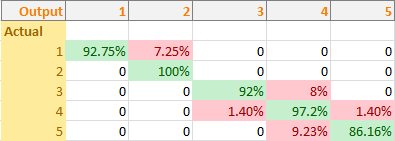
\includegraphics[width = 8cm, height = 3cm]{cof1_1}
%	\caption{Confusion Matrix of Masking Approach}
%\end{figure}
%
%\begin{figure}[h!]
%	\centering
%	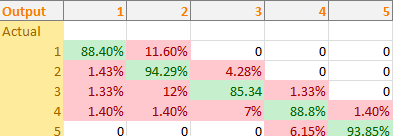
\includegraphics[width = 8cm, height = 3cm]{cof1_2}
%	\caption{Confusion Matrix of Method 2}
%\end{figure}

%colour
%\cellcolor{green}
\begin{table}[!h]
\caption{Confusion Matrix for Masking Approach}  
\begin{tabular}{ l *{5}{D{.}{.}{4}} }
\toprule
 & \multicolumn{5}{c}{\textbf{Predicted Class}} \\
\cmidrule(lr){2-6}
\textbf{Actual Class} & \multicolumn{1}{c}{G1} & \multicolumn{1}{c}{G2} & \multicolumn{1}{c}{G3} & \multicolumn{1}{c}{G4} & \multicolumn{1}{c}{G5} \\
\midrule
\texttt{G1} &0.9275  &  0.0725  & 0  & 0 & 0\\
\texttt{G2} &0  &  1  & 0  & 0 & 0\\ 
\texttt{G3} &0  &  0  & 0.92  & 0.08 & 0\\
\texttt{G4} &0  &  0  & 0.014  & 0.972 & 0.014\\
\texttt{G5} &0  &  0  & 0  & 0.0923 & 0.8616\\
        \bottomrule             
\end{tabular}
\end{table}


\begin{table}[!h]
\caption{Confusion Matrix for Gradient Approach}  
\begin{tabular}{ l *{5}{D{.}{.}{4}} }
\toprule
 & \multicolumn{5}{c}{\textbf{Predicted Class}} \\
\cmidrule(lr){2-6}
\textbf{Actual Class} & \multicolumn{1}{c}{G1} & \multicolumn{1}{c}{G2} & \multicolumn{1}{c}{G3} & \multicolumn{1}{c}{G4} & \multicolumn{1}{c}{G5} \\
\midrule
\texttt{G1} &0.884  &  0.116  & 0  & 0 & 0\\
\texttt{G2} &0.0143  &  0.9429  & 0.0428  & 0 & 0\\
\texttt{G3} &0.0133  &  0.12  & 0.8534  & 0.0133 & 0\\
\texttt{G4} &0.014  &  0.014  & 0.07  & 0.888 & 0.014\\
\texttt{G5} &0  &  0  & 0  & 0.0615 & 0.9385\\
        \bottomrule             
\end{tabular}
\end{table}
\subsection{OUR DATA-SET}
\begin{figure}[!h]
\begin{tabular}{ccccc}
\subfloat[G1]{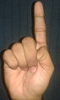
\includegraphics[width = 0.55in]{geo1}} &
\subfloat[G2]{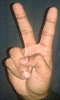
\includegraphics[width = 0.55in]{geo2}} &
\subfloat[G3]{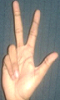
\includegraphics[width = 0.55in]{geo3}} &
\subfloat[G4]{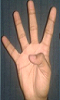
\includegraphics[width = 0.55in]{geo4}} &
\subfloat[G5]{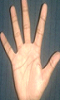
\includegraphics[width = 0.55in]{geo5}}
\end{tabular}
\caption{Hand Gestures used from our created dataset}
\end{figure}

To have an understanding of real\- time results, we collect our database of images and further test the accuracy. Ten pictures of ten different individuals were taken. The skin segments taken to train our Gaussian skin model were randomly taken from the skin samples of people of various ethnicity and region like North Indians, South Indians, North \- East Indians to test the robustness of our algorithm.

Accuracy by Masking Approach : - 96\%

Accuracy by Gradient Approach : - 98\%

\begin{table}[h!]
\caption{Confusion Matrix for Masking Approach}  
\begin{tabular}{ l *{5}{D{.}{.}{4}} }
\toprule
 & \multicolumn{5}{c}{\textbf{Predicted Class}} \\
\cmidrule(lr){2-6}
\textbf{Actual Class} & \multicolumn{1}{c}{G1} & \multicolumn{1}{c}{G2} & \multicolumn{1}{c}{G3} & \multicolumn{1}{c}{G4} & \multicolumn{1}{c}{G5} \\
\midrule
\texttt{G1} &1  &  0  & 0  & 0 & 0\\
\texttt{G2} &0  &  0.9  & 0.1  & 0 & 0\\ 
\texttt{G3} &0  &  0  & 1  & 0 & 0\\
\texttt{G4} &0  &  0  & 0  & 1 & 0\\
\texttt{G5} &0  &  0  & 0  & 0.3 & 0.7\\
        \bottomrule             
\end{tabular}
\end{table}


\begin{table}[h!]
\caption{Confusion Matrix for Gradient Approach}  
\begin{tabular}{ l *{5}{D{.}{.}{4}} }
\toprule
 & \multicolumn{5}{c}{\textbf{Predicted Class}} \\
\cmidrule(lr){2-6}
\textbf{Actual Class} & \multicolumn{1}{c}{G1} & \multicolumn{1}{c}{G2} & \multicolumn{1}{c}{G3} & \multicolumn{1}{c}{G4} & \multicolumn{1}{c}{G5} \\
\midrule
\texttt{G1} &1  &  0  & 0  & 0 & 0\\
\texttt{G2} &0  &  1  & 0  & 0 & 0\\
\texttt{G3} &0  &  0  & 1  & 0 & 0\\
\texttt{G4} &0  &  0  & 0  & 1 & 0\\
\texttt{G5} &0  &  0  & 0  & 0.3 & 0.7\\
        \bottomrule             
\end{tabular}
\end{table}



%\begin{figure}[h!]
%	\centering
%	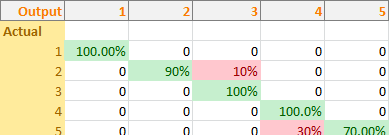
\includegraphics[width = 8cm, height = 3cm]{cof2_1}
%	\caption{Confusion Matrix of Masking Approach}
%\end{figure}
%
%
%\begin{figure}[h!]
%	\centering
%	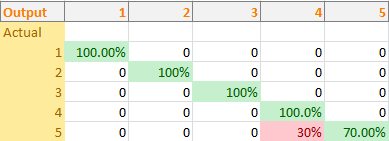
\includegraphics[width = 8cm, height = 3cm]{cof2_2}
%	\caption{Confusion Matrix of Method 2}
%\end{figure}
%

\begin{table}[h!]
\caption{Comparison of various methods}
\begin{center}
\begin{tabular}{|c|c|c|c|c|c|c|}
\hline
Method for feature extraction and classifier used & Average Accuracy \\ \hline
Bayes classifier \cite{Avraam2014StaticGR} & 83.40\% \\ \hline
PCA & 72.73\% \\ \hline
Kumar's Autoencoders \cite{kumar2014static} & 83.36\% \\ \hline
\textbf{Masking Approach} & 93.62\% \\ \hline
\textbf{Gradient Approach} & 90.13\% \\ \hline
\end{tabular}
\end{center}
\end{table}


\section{Conclusion and Future Scope}
This paper deals with two algorithms to understand the hand gestures and also compares their performances with each other as well as established methods \cite{khan2012hand}. In our work, we use the geometry of the hand for the recognition of hand gesture. It is a traditional type of algorithm and is thus robust.The proposed methods do not need any training phase \cite{7813732} to classify the hand gestures so is better than neural networks.

Sign Language Recognition, Robot Control automation of home appliances and presentation control are few of many applications of hand gesture recognition systems. Usage of hand gestures can be extended to control real time applications like pdf reader, VLC media player, paint, and so forth. This wireless control of embedded instruments is a significant progress towards the field of embedded vision and automation.

% conference papers do not normally have an appendix

\bibliographystyle{ieeetran}
\bibliography{references}

%\begin{thebibliography}{1}
%
%\bibitem{IEEEhowto:1199054}
%Simei G. Wysoski, Marcus V. Lamar, Susumu Kuroyanagi, Akira Iwata, (2002)\emph{"A Rotation
%Invariant Approach On Static-Gesture Recognition Using Boundary Histograms And Neural Networks"}, IEEE Proceedings of the 9th International Conference on Neural Information
%Processing, Singapura.
%
%\bibitem{IEEEhowto:Murakami:1991:GRU:108844.108900}
%Kouichi M., Hitomi T. (1999) \emph{"Gesture Recognition using Recurrent Neural Networks"}, ACM
%conference on Human factors in computing systems: Reaching through technology (CHI '91), pp.
%237-242. doi: 10.1145/108844.108900
%
%\bibitem{IEEEhowto:Freeman}
%W. T. Freeman and Michal R., (1995) \emph{"Orientation Histograms for Hand Gesture Recognition"}, IEEE International Workshop on Automatic Face and Gesture Recognition
%
%\bibitem{IEEEhowto:Sanz}
%Pablo Revuelta Sanz, Belén Ruiz Mezcua and José M. Sánchez Pena\emph{"” Depth Estimation – An Introduction"}
%
%\bibitem{IEEEhowto:Vishwakarma}
%D.K.~Vishwakarma and Rajiv Kapoor, \emph{"An Efficient Interpretation of Hand Gestures to Control Smart Interactive Television"}, International Journal of Computational Vision and Robotics, July, 2015,Impact Factor: 0.22, (In Press), (Pub.: Inderscience, UK).
%
%\bibitem{IEEEhowto:http}
%http://homepages.inf.ed.ac.uk/rbf/HIPR2/matmorph.htm
%
%\bibitem{IEEEhowto:ram}
%Ram Rajesh J, Nagarjunan D, Arunachalam RM and Aarthi R, \emph{"Distance Transform Based Hand Gestures Recognition For Powerpoint Presentation Navigation "}, Advanced Computing: An International Journal ( ACIJ ), Vol.3, No.3, May 2012
%
%\bibitem{IEEEhowto:Vishwakarma}
%D.K.~Vishwakarma; Maheshwari, Rockey ; Kapoor, Rajiv,  \emph{"An Efficient Approach for the Recognition of Hand Gestures from Very Low Resolution Images"},in 5th IEEE International Conference on Communication Systems and Network Technologies (CSNT), Gwalior, MP, pp.467-471, April 2015. DOI: 10.1109/CSNT.2015.84.
%
%
%\bibitem{IEEEhowto:Vishwakarma}
%D.K.~Vishwakarma and Rajiv Kapoor, \emph{"Simple and Intelligent system to recognize the expression of speech disabled person"}, 4th IEEE international conference on Intelligent Human Computer Interaction, pp: 1-6, 27th to 29th December, 2012, Kharagpur India, DOI:10.1109/IHCI.2012.6481804.
%
%
%\bibitem{IEEEhowto:massey}
%A.L.C. Barczak, N.H. Reyes, M. Abastillas, A. Piccio and T. Susnjak IIMS,Massey University, Auckland, New Zealand  \emph{"A New 2D Static Hand Gesture Colour Image Dataset for ASL Gestures"}, Res. Lett. Inf. Math. Sci., 2011, Vol. 15, pp. 12?20
%
%\bibitem{IEEEhowto:Avraam}
%Marimpis Avraam’s  \emph{"Static Gesture Recognition Combining Graph and Appearance Features"}, International Journal of Advanced Research in Artificial Intelligence,Vol. 3, No. 2, 2014
%
%
%\bibitem{IEEEhowto:Nandi}
%Kumar, Varun, Nandi, G. C. and Rahul, K \emph{"Static Hand Gesture
%Recognition Using Stacked Denoising Sparse Autoencoders
%"}, IEEE International Conference on Contemporary Computing, 2014.
%
%
%\bibitem{IEEEhowto:Khan}
%Rafiqul Zaman Khan and Noor Adnan Ibraheem, \emph{"Hand Gesture Recognition:   A Literature review"}, International Journal of Artificial Intelligence \& Applications (IJAIA), Vol.3, No.4, July 2012
%
%
%\bibitem{IEEEhowto:Vishwakarma}
%D.K.~Vishwakarma, Pridarshani and  Kuldeep Singh,  \emph{"A framework for the recognition of hand gesture in static postures"},in IEEE Conf. on Computing Communication and Automation, Greater Noida, UP, 2016, pp. 294-298. DOI:10.1109/CCAA.2016.7813732.
%
%\bibitem{IEEEhowto:Droeschel}
%D. Droeschel, J. Stückler, and S. Behnke,  \emph{"Learning to interpret
%pointing gestures with a time-of-flight camera"},in Proc. Int. Conf.
%Human-Robot Interact., Mar. 2011, pp. 481–488.
%
%\bibitem{IEEEhowto:Shotton}
%J. Shotton et al.,  \emph{"Real-time human pose recognition in parts from
%single depth images"},in Proc. IEEE CVPR, Jun. 2011, pp. 1297–1304.
%
%\bibitem{IEEEhowto:Regenbrecht}
%H. Regenbrecht, J. Collins, and S. Hoermann,  \emph{"A leap-supported,
%hybrid AR interface approach"},in Proc. Austral. Comput.-Human
%Interact. Conf., 2013, pp. 281–284
%
%\bibitem{IEEEhowto:Cheng}
%Hong Cheng, Senior Member, IEEE, Lu Yang, Member, IEEE, and Zicheng Liu, Fellow, IEEE,  \emph{"Survey on 3D Hand Gesture Recognition"}
%
%REFERENCE:
%
%
%
%\end{thebibliography}
%
%


% that's all folks
\end{document}


